\clearpage
\subsection{Declaring Variables (with custom types)} % (fold)
\label{sub:declaring_variables_with_custom_types_}

The custom types allow you to specify a data format. To make use of this format you must declare variables that use this type. The type can be used to declare \nameref{sub:local_variable}s and \nameref{sub:parameter}s, allowing you to store values in this format and pass the around between your functions and procedures.

\begin{figure}[h]
   \centering
   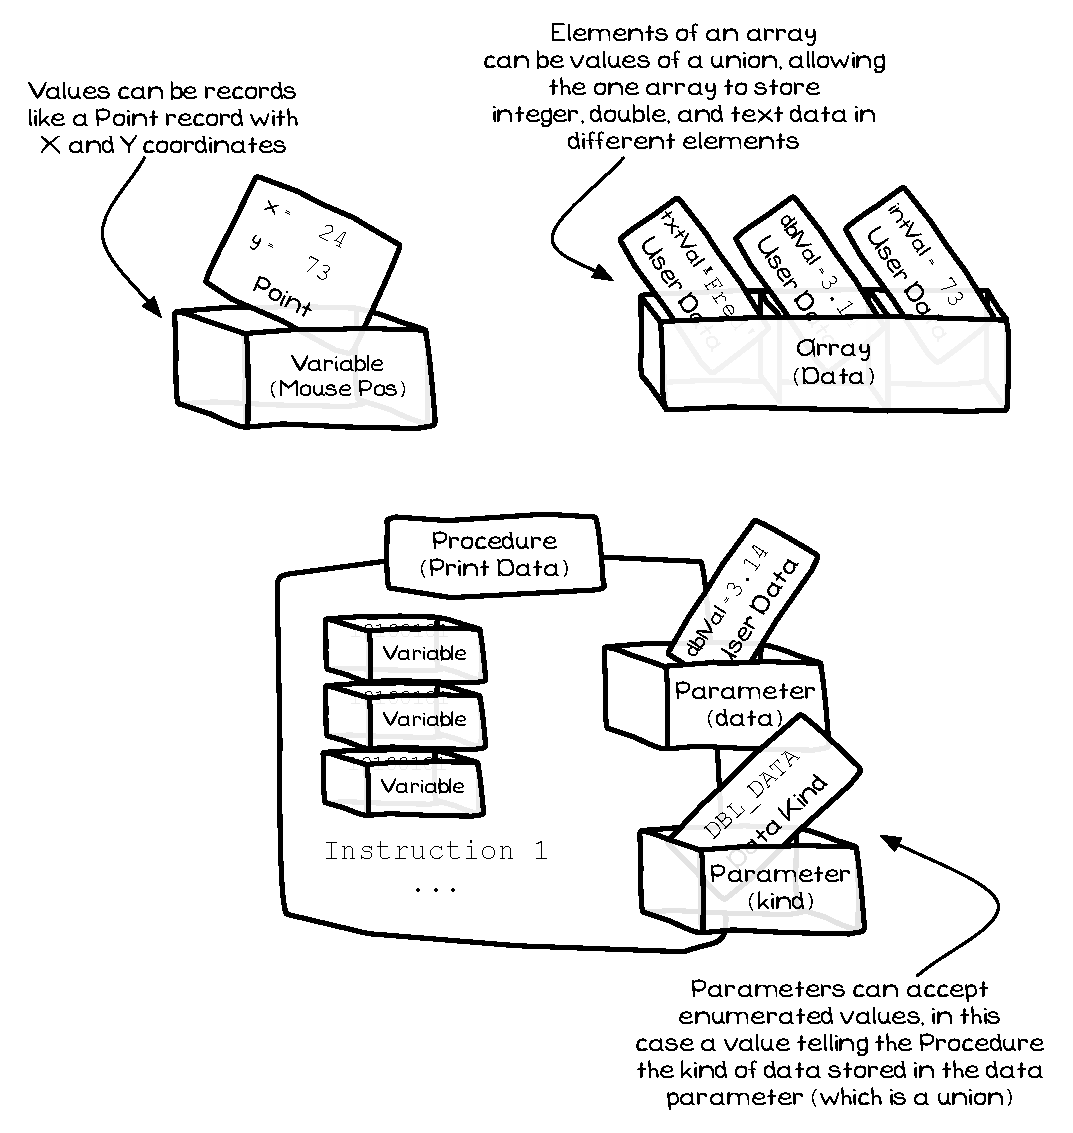
\includegraphics[width=0.87\textwidth]{./topics/type-decl/diagrams/VariableDeclaration} 
   \caption{Some examples of how you can use your types to declare the kind of data stored in variables}
   \label{fig:type-decl-variable-decl}
\end{figure}

\mynote{
\begin{itemize}
  \item Variables declaration is the \textbf{term} given to the code that creates Variables.
  \item The Variables you create store data as described in your custom type definitions.
  \item In \fref{fig:type-decl-variable-decl} there are the following examples:
  \begin{itemize}
    \item \texttt{Mouse Pos}: A Variable that stores \texttt{Point} \nameref{ssub:record} data.
    \item \texttt{Data}: \nameref{sub:array} that stores \texttt{User Data} values which are either integer, double, or text values using a \nameref{ssub:union}.
    \item \texttt{kind}: \nameref{sub:parameter} that passes in an \nameref{ssub:enum} value from the \texttt{Data Kind} type. This value can then be used by 
  \end{itemize}
  \item You can combine these types in a huge variety of ways. The best idea is to try and model the entities related to your program. 
\end{itemize}
}


% subsection declaring_variables_with_custom_types_ (end)